\section{Data Architecture}

Each service has its own database, schema and credentials. Cross-service
references (\texttt{reservation\_id}, \texttt{listing\_id}, \texttt{user\_id},
\texttt{zone\_id}\ldots) are logical, never foreign keys. Every service that
publishes or consumes events also keeps an \texttt{outbox\_event} table
(\texttt{event\_id}, \texttt{type}, \texttt{payload}, \texttt{published\_at})
and a \texttt{processed\_event} table keyed by (\texttt{event\_id},
\texttt{consumer}); they are not repeated below.

\subsection{Storage Type}

The storage of each work stream is chosen by its access pattern and integrity
needs (Table~\ref{tab:storage}). Relational storage is used wherever the
database must enforce a business rule.

\begin{longtable}{@{}L{3.6cm}L{3.2cm}L{7.0cm}@{}}
\toprule
\textbf{Data (owner)} & \textbf{Storage} & \textbf{Rationale} \\
\midrule
\endhead
\multicolumn{3}{@{}l}{\emph{Payments and Refunds}} \\
Payments, attempts, refunds, idempotency records, inbox (Payment Coord.) &
  Relational &
  Unique payment per reservation; refunded $\leq$ captured. Idempotency
  records commit with the payment change; a cache could lose keys, the same
  reason Airbnb gives~\cite{airbnb-orpheus}. \\
Ledger and payouts (Ledger \& Payout) & Relational, append-only &
  Every journal transaction balances; auditors need joins and totals. \\
\addlinespace
\multicolumn{3}{@{}l}{\emph{Reservation and Calendar}} \\
Accommodations, calendar, reservations, agreements & Relational (PostgreSQL) &
  The exclusion constraint and the reservation change commit together; no
  cache in front of availability. Hold timers are rebuildable from
  \texttt{hold\_expires\_at}. \\
\addlinespace
\multicolumn{3}{@{}l}{\emph{Pricing Engine}} \\
Model versions, zone snapshot (Pricing) & Relational &
  One \texttt{ACTIVE} version (partial unique index); the request is a single
  key read. \\
Calculation history (Pricing) & Document store; object storage after 1 year &
  Append-only, self-contained documents; cheap archive for audit and model
  training. \\
Search counters, demand snapshots (Demand) & Key-value / time-series &
  One increment per search event on \texttt{zone\_id\#day}; rebuildable. \\
Context events (Context) & Relational &
  Monthly batch; unique key avoids duplicates on re-runs. \\
\addlinespace
\multicolumn{3}{@{}l}{\emph{Identity, Communication and Internal Operations}} \\
Credentials, sessions, keys (Identity) & Dedicated identity store &
  Password material isolated; key rotation and immediate revocation. \\
Profiles, roles; cases; admin actions & Relational &
  Transactional changes and queries over related records. \\
Messages (Messaging) & Document or wide-column &
  High volume, ordered and partitioned by \texttt{conversationId}. \\
Attachments (Messaging) & Object storage & Served by short-lived URLs. \\
Preferences, devices, attempts (Notification) & Key-value / document &
  Point lookups; TTL on duplicate-suppression keys. \\
Audit records (Audit) & Append-only immutable store + search index &
  Tamper-evident; the index is derived and rebuildable. \\
\bottomrule
\caption{Storage type per work stream.}
\label{tab:storage}
\end{longtable}

Money is stored as an integer amount plus a currency code (e.g.\
\texttt{1070000 COP}). Passwords are stored only as salted hashes, and message
bodies and payment data never appear in events, logs or audit payloads. Logs,
metrics and traces live in an observability platform and are never audit
evidence.

\subsection{Data Model}

% ------------------------- Payments and Refunds -------------------------
\begingroup
\setlength{\emergencystretch}{3em}
\subsubsection{Payments and Refunds}
\label{sec:pay-model}

\begin{longtable}{@{}L{3.4cm}L{10.4cm}@{}}
\toprule
\textbf{Table} & \textbf{Main columns and constraints} \\
\midrule
\endhead
\multicolumn{2}{@{}l}{\emph{Payments DB}} \\
\texttt{payment} & \texttt{payment\_id} (PK), \texttt{reservation\_id}
  (unique), \texttt{guest\_id}, \texttt{host\_id}, \texttt{amount},
  \texttt{captured\_amount}, \texttt{refunded\_amount} (check $\leq$
  captured), \texttt{currency}, \texttt{price\_snapshot}, \texttt{status},
  \texttt{version}. \\
\texttt{payment\_attempt} & \texttt{attempt\_id} (PK, also gateway
  idempotency key), \texttt{payment\_id}, \texttt{attempt\_no},
  \texttt{method\_token}, \texttt{status}, \texttt{decline\_code}. \\
\texttt{refund} & \texttt{refund\_id} (PK), \texttt{payment\_id},
  \texttt{amount}, \texttt{source} (\texttt{CANCELLATION}, \texttt{SUPPORT}),
  \texttt{support\_case\_id}, \texttt{funded\_by}, \texttt{status},
  \texttt{idempotency\_key} (unique). \\
\texttt{idempotency\_record} & \texttt{key} (PK), \texttt{request\_hash},
  \texttt{state}, stored response, \texttt{expires\_at}. \\
\texttt{gateway\_event\_inbox} & Webhooks keyed by gateway event id. \\
\addlinespace
\multicolumn{2}{@{}l}{\emph{Ledger DB}} \\
\texttt{account} & \texttt{account\_id} (PK), \texttt{type}
  (\texttt{GATEWAY\_CLEARING}, \texttt{HOST\_PAYABLE},
  \texttt{PLATFORM\_MARGIN}, \texttt{GOODWILL\_EXPENSE}), \texttt{owner\_id}. \\
\texttt{journal\_txn} & \texttt{txn\_id} (PK), \texttt{source\_event\_id}
  (unique), \texttt{type}, \texttt{reservation\_id}. \\
\texttt{ledger\_entry} & \texttt{txn\_id}, \texttt{account\_id},
  \texttt{direction}, \texttt{amount}; debits equal credits per transaction. \\
\texttt{payout} & \texttt{payout\_id} (PK), \texttt{host\_id},
  \texttt{amount}, \texttt{release\_at}, \texttt{status},
  \texttt{idempotency\_key} (unique). \\
\bottomrule
\caption{Main tables of Payments and Refunds.}
\label{tab:pay-model}
\end{longtable}

\paragraph{Money split.} The guest is charged once. With the frozen snapshot,
$\textit{HostAmount} = \textit{basePrice} \times \textit{nights}$ and
$\textit{PlatformMargin} = (\textit{multiplier} - 1) \times
\textit{basePrice} \times \textit{nights}$. For reservation
\texttt{res-9f3a21} (4 nights at 250{,}000 COP, multiplier 1.07) the guest pays
1{,}070{,}000 COP: 1{,}000{,}000 for the host and 70{,}000 of margin. The
capture produces this journal transaction:

{\footnotesize
\begin{verbatim}
{ "txn_id": "jt-10044", "source_event_id": "e-7c22d1", "type": "CAPTURE",
  "reservation_id": "res-9f3a21", "currency": "COP", "entries": [
  {"account":"GATEWAY_CLEARING","direction":"DEBIT","amount":1070000},
  {"account":"HOST_PAYABLE:host-678","direction":"CREDIT","amount":1000000},
  {"account":"PLATFORM_MARGIN","direction":"CREDIT","amount":70000} ] }
\end{verbatim}
}

A refund is a reverse transaction; if the platform funds it, it debits
\texttt{GOODWILL\_EXPENSE} instead of the host. A refund after payout leaves
the host balance negative and is recovered from later payouts.
\endgroup

% ------------------------- Reservation and Calendar -------------------------
\subsubsection{Reservation and Calendar}
\label{sec:res-model}

\begin{table}[!ht]
  \centering
  \small
  \begin{tabularx}{\textwidth}{@{}>{\raggedright\arraybackslash}p{4.2cm}>{\raggedright\arraybackslash}X@{}}
    \toprule
    \textbf{Table} & \textbf{Main columns} \\
    \midrule
    \texttt{accommodation} & \texttt{listing\_id} (PK), \texttt{host\_id}, \texttt{zone\_id}, \texttt{max\_guests}, \texttt{base\_price}, \texttt{includes\_cleaning}, \texttt{multiplier}, \texttt{effective\_nightly\_rate}, \texttt{status}, \texttt{version} \\
    \texttt{reservation} & \texttt{reservation\_id} (PK), \texttt{listing\_id}, \texttt{guest\_id}, dates, \texttt{guests\_count}, \texttt{status}, \texttt{hold\_expires\_at}, \texttt{total\_amount}, \texttt{price\_snapshot}, \texttt{idempotency\_key}, \texttt{version} \\
    \texttt{calendar\_entry} & \texttt{entry\_id} (PK), \texttt{listing\_id}, \texttt{period} (\texttt{daterange}), \texttt{kind} (\texttt{HOLD}, \texttt{RESERVATION}, \texttt{HOST\_BLOCK}), \texttt{reservation\_id}, \texttt{expires\_at}, \texttt{released\_at} \\
    \texttt{checkin\_agreement} & \texttt{reservation\_id} (unique), check-in/out times, \texttt{status} \\
    \texttt{reservation\_status\_history} & \texttt{reservation\_id}, \texttt{from\_status}, \texttt{to\_status}, \texttt{actor}, \texttt{reason} \\
    \bottomrule
  \end{tabularx}
  \caption{Data model of the Reservation and Accommodation Service.}
\end{table}

\noindent Reservation states: \texttt{PENDING\_PAYMENT}, \texttt{CONFIRMED},
\texttt{PAYMENT\_FAILED}, \texttt{EXPIRED} and \texttt{CANCELLED}.

% ------------------------- Pricing Engine -------------------------
\begingroup
\setlength{\emergencystretch}{3em}
\subsubsection{Pricing Engine}
\label{sec:price-model}

\begin{figure}[H]
  \centering
  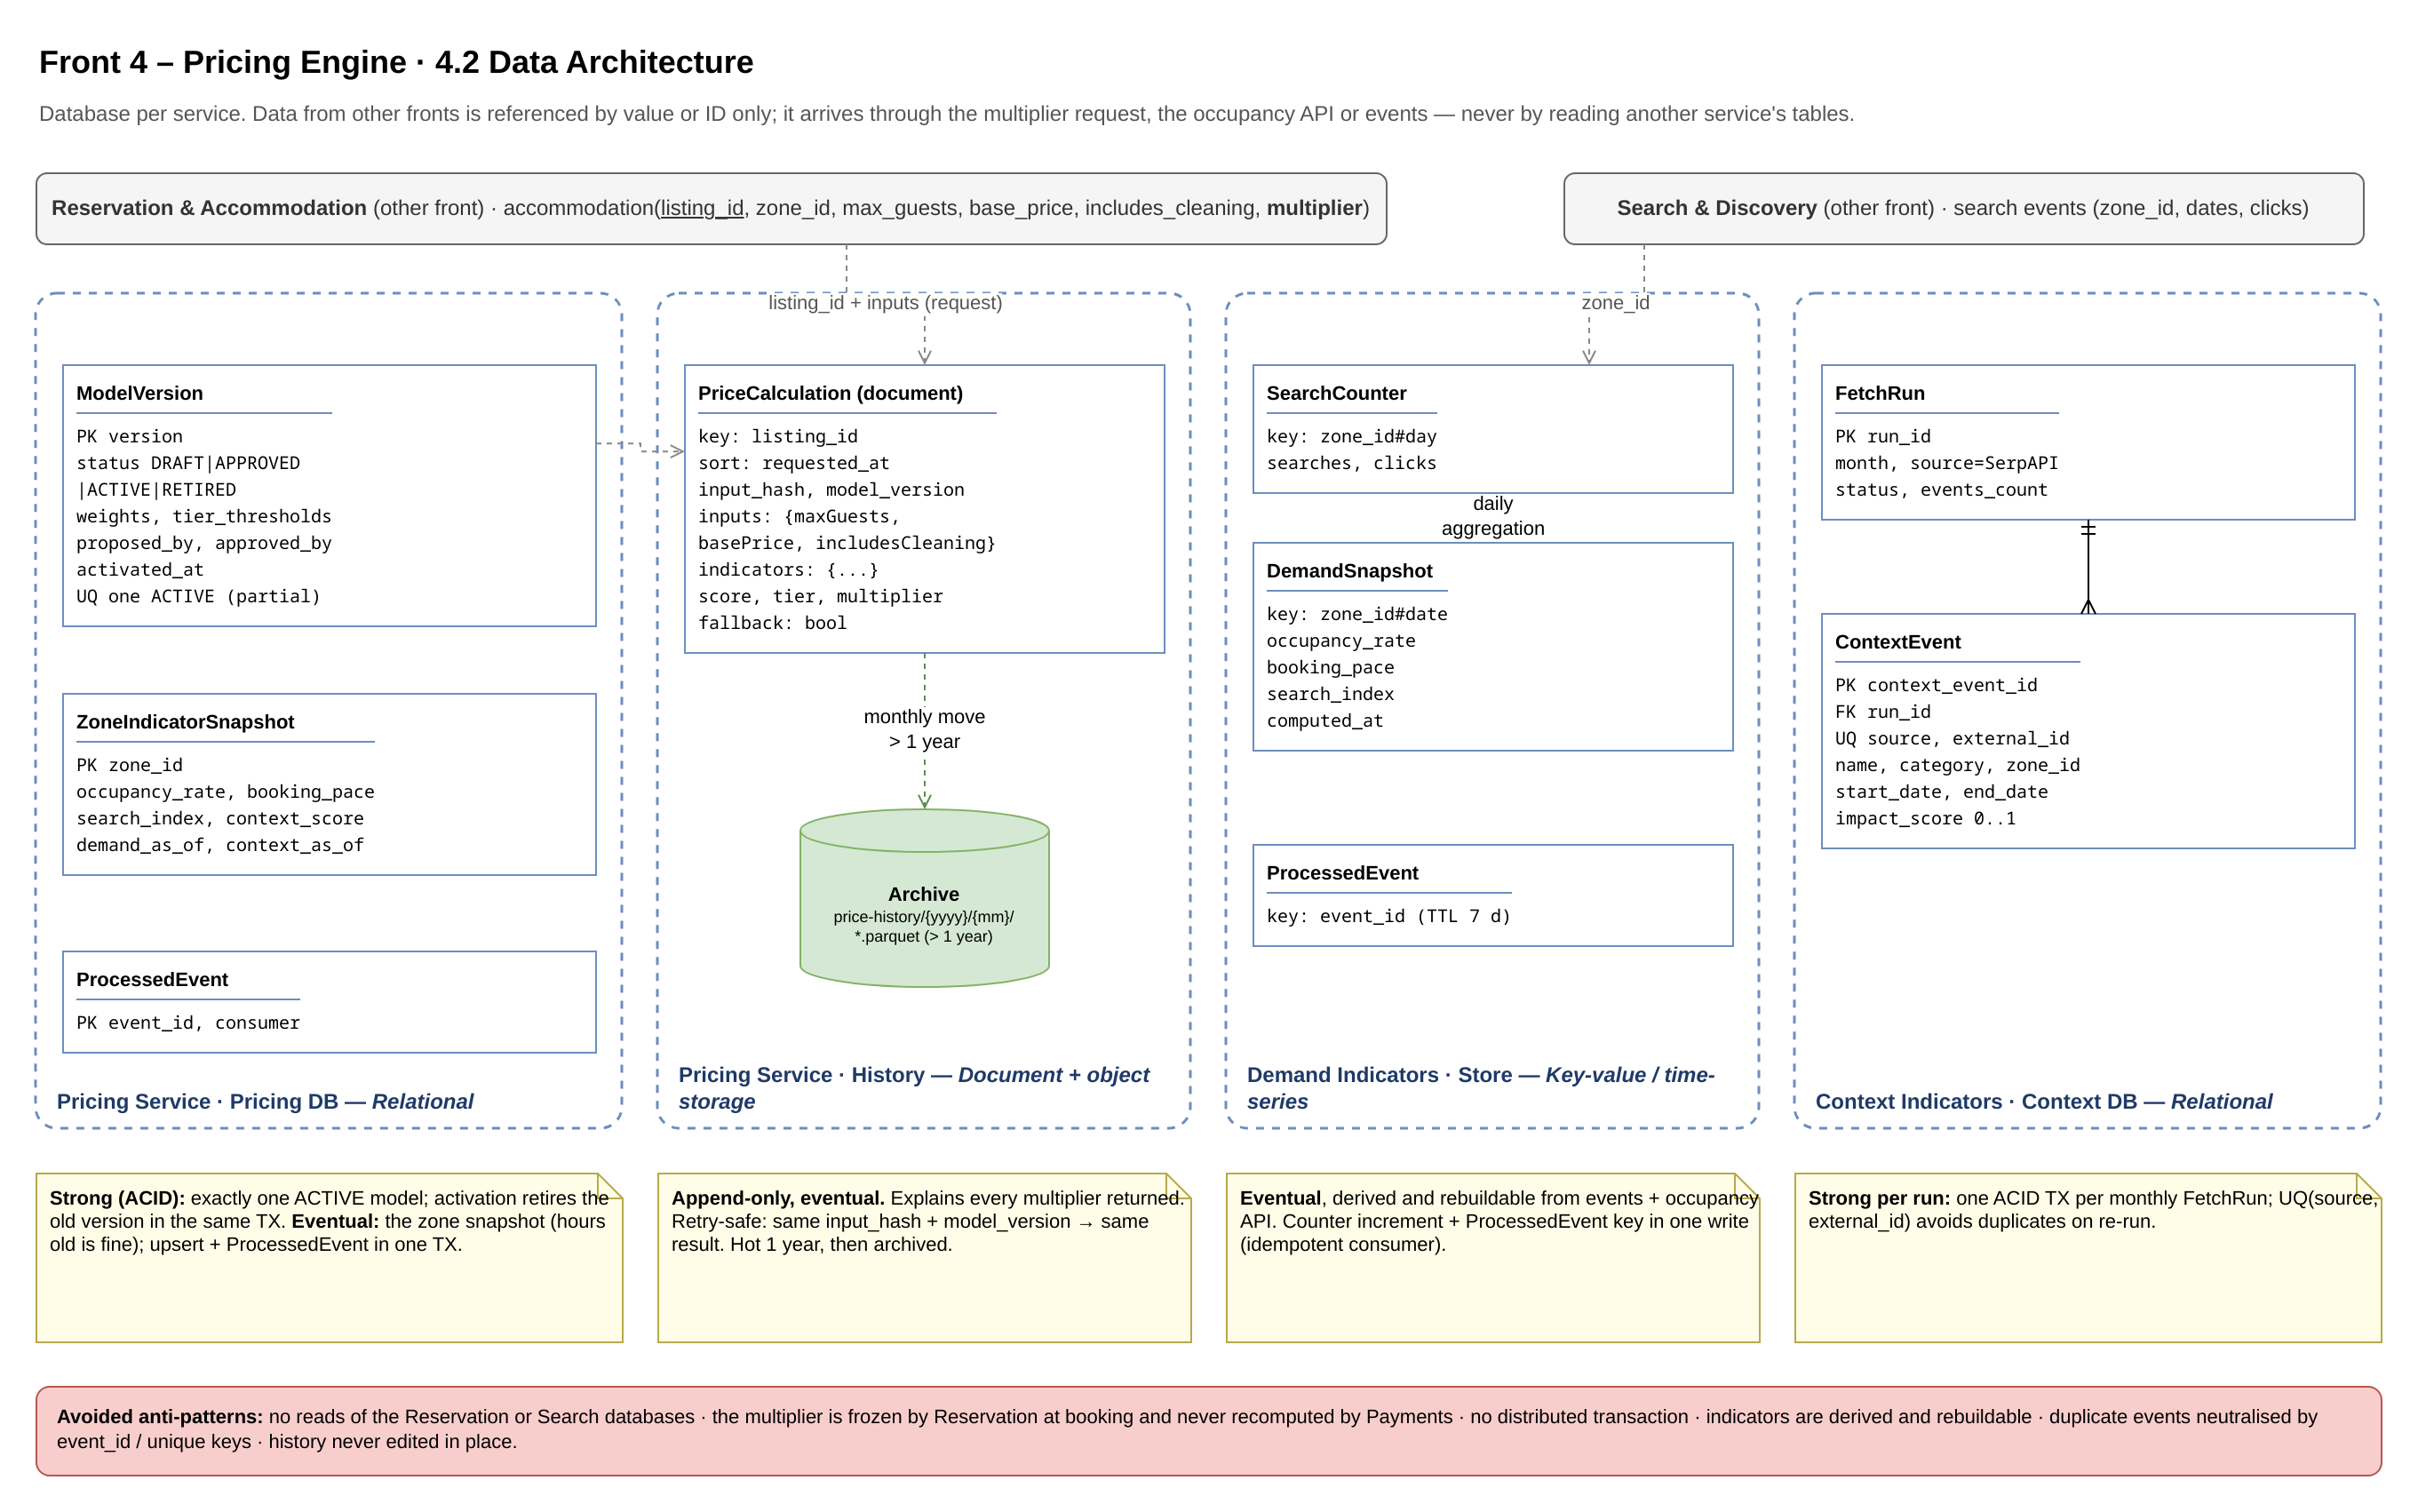
\includegraphics[width=\linewidth]{images/pricing_42_data_architecture.png}
  \caption{Pricing Engine data: owner, storage and main entities.}
  \label{fig:price-data}
\end{figure}

\begin{longtable}{@{}L{3.8cm}L{10.0cm}@{}}
\toprule
\textbf{Entity (store)} & \textbf{Main fields and constraints} \\
\midrule
\endhead
\texttt{model\_version} (Pricing DB) & \texttt{version} (PK), \texttt{status}
  (\texttt{DRAFT}, \texttt{APPROVED}, \texttt{ACTIVE}, \texttt{RETIRED}),
  \texttt{weights}, \texttt{tier\_thresholds}, \texttt{approved\_by};
  unique partial index on \texttt{ACTIVE}. \\
\texttt{zone\_indicator\_snapshot} (Pricing DB) & \texttt{zone\_id} (PK),
  \texttt{occupancy\_rate}, \texttt{booking\_pace}, \texttt{search\_index},
  \texttt{context\_score}, \texttt{as\_of} dates. \\
\texttt{PriceCalculation} (history) & Key \texttt{listing\_id} +
  \texttt{requested\_at}; inputs, indicators, \texttt{model\_version},
  \texttt{score}, \texttt{tier}, \texttt{multiplier}, \texttt{fallback}. \\
\texttt{SearchCounter}, \texttt{DemandSnapshot} (Demand) & Keys
  \texttt{zone\_id\#day}; searches, clicks; occupancy, pace, search index. \\
\texttt{fetch\_run}, \texttt{context\_event} (Context) & Run per month;
  event with \texttt{source} + \texttt{external\_id} (unique),
  \texttt{zone\_id}, dates, \texttt{impact\_score}. \\
\bottomrule
\caption{Main entities of the Pricing Engine.}
\label{tab:price-model}
\end{longtable}
\endgroup

% ------------------------- Identity, Communication and Internal Operations -------------------------
\begingroup
\setlength{\emergencystretch}{3em}
\subsubsection{Identity, Communication and Internal Operations}
\label{sec:id-model}

\begin{longtable}{@{}L{3.0cm}L{10.8cm}@{}}
\toprule
\textbf{Store} & \textbf{Main entities and key fields} \\
\midrule
\endhead
Identity & \texttt{Credential} (\texttt{passwordHash}, \texttt{status}),
  \texttt{Session} (\texttt{refreshTokenHash}, \texttt{expiresAt},
  \texttt{revokedAt}), \texttt{MfaFactor}, \texttt{SigningKey},
  \texttt{RevocationEntry}. \\
Profile & \texttt{User} (\texttt{email} unique, \texttt{accountStatus}),
  \texttt{RoleAssignment} (one active role per user). \\
Messaging & \texttt{Conversation}, \texttt{Message} (partition
  \texttt{conversationId}, sort \texttt{messageId}), \texttt{ReadState},
  \texttt{Attachment}. \\
Notification & \texttt{Notification} (unique \texttt{(eventId, userId,
  channel)}, \texttt{status}, \texttt{attempts}), \texttt{Preference},
  \texttt{Device}, \texttt{Template}. \\
Support & \texttt{SupportCase} (\texttt{status}, \texttt{assigneeId},
  \texttt{version}), \texttt{CaseComment}, \texttt{CaseTransition}. \\
Administration & \texttt{AdminAction} (\texttt{actionType},
  \texttt{targetId}, \texttt{reason}, \texttt{stepUpVerified}),
  \texttt{Approval}, \texttt{Policy}. \\
Audit & \texttt{AuditRecord} (\texttt{sequence} unique, \texttt{actorId},
  \texttt{action}, \texttt{resourceId}, \texttt{prevHash},
  \texttt{recordHash}, \texttt{signature}), \texttt{AuditAnchor}
  (\texttt{merkleRoot}). \\
\bottomrule
\caption{Main entities of Identity, Communication and Internal Operations.}
\label{tab:id-model}
\end{longtable}

A message is \texttt{SENT}, \texttt{DELIVERED} or \texttt{READ}; a
notification is \texttt{QUEUED}, \texttt{SENDING}, \texttt{SENT\_TO\_PROVIDER},
\texttt{DELIVERED}, \texttt{FAILED} or \texttt{SUPPRESSED}; a support case is
\texttt{OPEN}, \texttt{IN\_PROGRESS}, \texttt{WAITING\_FOR\_USER},
\texttt{RESOLVED} or \texttt{CLOSED}. Each audit record stores the hash of the
previous one, so altering a record breaks every later hash; a signed Merkle
anchor per period lets an auditor verify any range.
\endgroup

\subsection{Consistency Requirements}

Data that guards money, availability or security is strongly consistent;
everything derived from events (search index, notifications, audit index,
indicator snapshots) is eventually consistent. Table~\ref{tab:consistency}
lists the specific cases.

\begin{longtable}{@{}L{3.6cm}L{3.2cm}L{7.0cm}@{}}
\toprule
\textbf{Data} & \textbf{Consistency} & \textbf{Why} \\
\midrule
\endhead
\multicolumn{3}{@{}l}{\emph{Payments and Refunds}} \\
Payment state & Strong; exactly-once effect &
  Never charge twice: idempotency from caller, to the gateway (attempt id
  stored before the call) and on events. \\
Ledger & Strong, append-only & Balanced; \texttt{source\_event\_id} unique. \\
Gateway & Reconciled & Webhooks, 5-minute reconciler, daily settlement
  comparison. \\
\addlinespace
\multicolumn{3}{@{}l}{\emph{Reservation and Calendar}} \\
Calendar and reservations & Strong & Overlapping active entries are
  impossible under concurrency. \\
Reservation + payment + ledger & Eventual (seconds), saga & Confirmed only
  after a valid payment result; late payments recovered or refunded. \\
Price and conditions & Frozen at booking & Later host edits never alter a
  reservation (FR02). \\
\addlinespace
\multicolumn{3}{@{}l}{\emph{Pricing Engine}} \\
Active model version & Strong & Two requests are never priced with different
  active versions. \\
Zone snapshot & Eventual (hours) & Demand changes slowly; yesterday's data is
  enough for a margin tier. \\
\addlinespace
\multicolumn{3}{@{}l}{\emph{Identity, Communication and Internal Operations}} \\
Credentials, sessions, roles & Strong & Revocations and role changes take
  effect at once; token claims may lag only within the short token
  lifetime. \\
Messages & Strong per conversation & Ordering matters; read state across
  devices may lag. \\
Support cases & Strong per case & Optimistic concurrency on
  \texttt{version}. \\
Audit records & Durable before acknowledging & Evidence must exist before
  the action is confirmed. \\
\bottomrule
\caption{Consistency requirements.}
\label{tab:consistency}
\end{longtable}

\subsection{Transactional Boundaries}

Every state change commits in one local ACID transaction together with its
outbox event and, for consumers, its processed-event mark. Nothing spans two
databases: cross-service workflows are sagas. The boundaries that need
specific attention are:
\begin{itemize}
  \item \textbf{Payments.} The attempt is stored \emph{before} calling the
    gateway. Compensations are \emph{void} before capture (free, immediate)
    and \emph{refund} after capture; a failed refund never undoes a
    cancellation. The gateway cannot join a transaction, so uncertain results
    stay \texttt{PENDING}. Each ledger transaction is balanced and committed
    atomically.
  \item \textbf{Reservation.} The hold releases expired holds, inserts the
    \texttt{HOLD} entry and the reservation in one transaction; confirmation,
    cancellation and expiration are conditional updates on the expected
    status. The Pricing call happens \emph{before} the listing transaction.
    Overlaps are rejected by the database:
\begin{lstlisting}[language=SQL, basicstyle=\ttfamily\footnotesize, frame=single]
ALTER TABLE calendar_entry ADD CONSTRAINT no_overlap
  EXCLUDE USING gist (listing_id WITH =, period WITH &&)
  WHERE (released_at IS NULL);
\end{lstlisting}
  \item \textbf{Pricing.} The multiplier request writes nothing but an
    appended history document; same inputs and version give the same result,
    so retries are harmless. Model activation retires the old version and
    activates the new one in one transaction, after the audit record.
  \item \textbf{Identity.} Registration is a saga: the credential stays
    pending until User Profile creates the profile. An administrative action
    appends an ``attempt'' record, calls the owner and appends the
    ``outcome''; if the owner fails, it is marked \texttt{FAILED} and
    compensated. Audit appends are idempotent by \texttt{recordId} and
    serialized to keep the hash chain.
\end{itemize}

\subsection{Shared Data Anti-patterns Avoided}

\begin{longtable}{@{}L{3.6cm}L{10.2cm}@{}}
\toprule
\textbf{Anti-pattern} & \textbf{How it is avoided} \\
\midrule
\endhead
Shared database & No service reads another's tables; Pricing reads occupancy
  through the calendar API and searches through events. \\
Dual writes & State and events are bound by the transactional outbox. \\
Distributed transactions or locks & Sagas, idempotency keys and
  compensations; double booking is prevented by the exclusion constraint, not
  by a lock. \\
Duplicated authority & The search index, the pricing snapshot and caches
  (roles, contact data, keys) are rebuildable projections; the owner stays
  authoritative. \\
Recomputing prices & Payments and Reservation use the frozen multiplier; the
  engine never re-prices an existing booking. \\
Synchronous fan-out & The multiplier request reads a local snapshot instead
  of calling indicator services or SerpAPI. \\
Mutable history & Ledger balances, pricing history and audit records are
  append-only; operational logs are never evidence. \\
Duplicate processing & Consumers store processed event IDs; notifications use
  the key \texttt{(eventId, userId, channel)}. \\
Sensitive data in copies & Only gateway tokens are stored; events carry IDs,
  not message bodies or payment data. \\
\bottomrule
\caption{Shared-data anti-patterns and how the design avoids them.}
\label{tab:antipatterns}
\end{longtable}

\paragraph{Security controls.} TLS on all traffic and encryption at rest;
keys and third-party credentials in dedicated secret stores; least privilege
per service identity for APIs and topics; short-lived access tokens, rotated
refresh tokens and session revocation on role change or suspension; MFA for
privileged roles plus step-up and a documented reason for sensitive actions;
no passwords, tokens, message bodies or payment data in logs.
